\documentclass[a4paper, justified]{tufte-handout}\usepackage[]{graphicx}\usepackage[]{xcolor}
% maxwidth is the original width if it is less than linewidth
% otherwise use linewidth (to make sure the graphics do not exceed the margin)
\makeatletter
\def\maxwidth{ %
  \ifdim\Gin@nat@width>\linewidth
    \linewidth
  \else
    \Gin@nat@width
  \fi
}
\makeatother

\definecolor{fgcolor}{rgb}{0.345, 0.345, 0.345}
\newcommand{\hlnum}[1]{\textcolor[rgb]{0.686,0.059,0.569}{#1}}%
\newcommand{\hlstr}[1]{\textcolor[rgb]{0.192,0.494,0.8}{#1}}%
\newcommand{\hlcom}[1]{\textcolor[rgb]{0.678,0.584,0.686}{\textit{#1}}}%
\newcommand{\hlopt}[1]{\textcolor[rgb]{0,0,0}{#1}}%
\newcommand{\hlstd}[1]{\textcolor[rgb]{0.345,0.345,0.345}{#1}}%
\newcommand{\hlkwa}[1]{\textcolor[rgb]{0.161,0.373,0.58}{\textbf{#1}}}%
\newcommand{\hlkwb}[1]{\textcolor[rgb]{0.69,0.353,0.396}{#1}}%
\newcommand{\hlkwc}[1]{\textcolor[rgb]{0.333,0.667,0.333}{#1}}%
\newcommand{\hlkwd}[1]{\textcolor[rgb]{0.737,0.353,0.396}{\textbf{#1}}}%
\let\hlipl\hlkwb

\usepackage{framed}
\makeatletter
\newenvironment{kframe}{%
 \def\at@end@of@kframe{}%
 \ifinner\ifhmode%
  \def\at@end@of@kframe{\end{minipage}}%
  \begin{minipage}{\columnwidth}%
 \fi\fi%
 \def\FrameCommand##1{\hskip\@totalleftmargin \hskip-\fboxsep
 \colorbox{shadecolor}{##1}\hskip-\fboxsep
     % There is no \\@totalrightmargin, so:
     \hskip-\linewidth \hskip-\@totalleftmargin \hskip\columnwidth}%
 \MakeFramed {\advance\hsize-\width
   \@totalleftmargin\z@ \linewidth\hsize
   \@setminipage}}%
 {\par\unskip\endMakeFramed%
 \at@end@of@kframe}
\makeatother

\definecolor{shadecolor}{rgb}{.97, .97, .97}
\definecolor{messagecolor}{rgb}{0, 0, 0}
\definecolor{warningcolor}{rgb}{1, 0, 1}
\definecolor{errorcolor}{rgb}{1, 0, 0}
\newenvironment{knitrout}{}{} % an empty environment to be redefined in TeX

\usepackage{alltt}
\geometry{
  left=24.8mm, % left margin
  textwidth=100mm, % main text block
  marginparsep=3mm, % gutter between main text block and margin notes
  marginparwidth=75mm % width of margin notes
}
% Packages {
  \usepackage[portuguese]{babel}
  % KableExtra {
    \usepackage{booktabs}
    \usepackage{longtable}
    \usepackage{array}
    \usepackage{multirow}
    \usepackage{wrapfig}
    \usepackage{float}
    \usepackage{colortbl}
    \usepackage{pdflscape}
    \usepackage{tabu}
    \usepackage{threeparttable}
    \usepackage{threeparttablex}
    \usepackage[normalem]{ulem}
    \usepackage{makecell}
    \usepackage{xcolor}
    \usepackage{comment}
    \usepackage{lipsum}
    \usepackage{tabulary}
    \usepackage{tabularx}
    % \usepackage{showframe}
  % }
% }



% Titulo {
  \title{TODO TITULO}
  \author{
    André Plancha, 105289 \\
    <Andre\_Plancha@iscte-iul.pt> \\
    Tomás Ribeiro, 105220 \\
    <tfroo1@iscte-iul.pt> \\
    Afonso Silva, 105208 \\
    <agsos@iscte-iul.pt> \\
    Rui Chaves, 104914 \\
    <rfpcs1@iscte-iul.pt>
  }
  \date{28/11/2022 \\ Versão 0.0.1} % 
% }

% { bug workaround (https://github.com/Tufte-LaTeX/tufte-latex/issues/64#issuecomment-78572017)
\renewcommand\allcapsspacing[1]{{\addfontfeature{LetterSpace=15}#1}}
\renewcommand\smallcapsspacing[1]{{\addfontfeature{LetterSpace=10}#1}}
% }
% {R code and table
\newenvironment{RTable}[1]{\begin{margintable}\begin{center}\begin{tabular}{#1}}{\end{tabular}\end{center}\end{margintable}}
\newenvironment{RTable*}[1]{\begin{table*}\begin{center}\begin{tabular}{#1}}{\end{tabular}\end{center}\end{table*}}
% }
\IfFileExists{upquote.sty}{\usepackage{upquote}}{}
\begin{document}



% cover { 
  \cleardoublepage
  {
  \sffamily
  \begin{fullwidth}
  \fontsize{18}{20}\selectfont\par\noindent\textcolor{darkgray}{\allcaps{\thanklessauthor}}%
  \vspace{11.5pc}
  \fontsize{36}{40}\selectfont\par\noindent\textcolor{darkgray}{\allcaps{\thanklesstitle}}%
  \vfill
  \fontsize{14}{16}\selectfont\par\noindent\allcaps{\thanklesspublisher}
  \end{fullwidth}
  }
  \thispagestyle{empty}
  \clearpage
% }
% abstract
  \newgeometry{left=30mm, right=107mm, textwidth=100mm}
  \vspace*{1cm}
  \begin{fullwidth}
    \Large{
      Hello 
      \lipsum[2]
      \vspace{5cm}
      \lipsum[3]
      \thispagestyle{empty}
    }
    \clearpage
  \end{fullwidth}
  \restoregeometry
% }
% descricao airbnb TODO
% also o airbnb n vende quartos
O nosso trabalho tem como objetivo desenvolver um modelo que permita prever o preço a que os quartos são colocados á venda no Airbnb. Com vista nesse objetivo foi nos disponibilizada uma base de dados que tem várias informações úteis para a realização desta tarefa.
Usámos como suporte técnico a linguagem R, através do uso de um computador pessoal quer para a limpeza de dados quer para o seu tratamento de dados e as respetivas previsões efectuadas.

\begin{knitrout}
\definecolor{shadecolor}{rgb}{0.969, 0.969, 0.969}\color{fgcolor}\begin{kframe}
\begin{alltt}
\hlstd{df} \hlkwb{<-} \hlkwd{read.csv}\hlstd{(}\hlkwd{here}\hlstd{(}\hlstr{"data"}\hlstd{,}
    \hlstr{"listings.csv"}\hlstd{))}
\hlstd{shape} \hlkwb{<-} \hlkwd{st_read}\hlstd{(}\hlkwd{here}\hlstd{(}\hlstr{"data"}\hlstd{,}
    \hlstr{"SF Planning Neighborhood Groups Map"}\hlstd{))}
\hlkwd{tmap_mode}\hlstd{(}\hlstr{"plot"}\hlstd{)}
\hlstd{shape_plot} \hlkwb{<-} \hlstd{shape} \hlopt
    \hlkwd{ggplot}\hlstd{()} \hlopt{+} \hlkwd{geom_sf}\hlstd{()} \hlopt{+}
    \hlkwd{theme}\hlstd{(}\hlkwc{legend.position} \hlstd{=} \hlstr{"bottom"}\hlstd{)}
\end{alltt}
\end{kframe}
\end{knitrout}

A base de dados que nos foi disponibilizada vem do  projeto \href{http://insideairbnb.com/}{Inside Airbnb}, fundado por Murray Cox com a missão de "[...] fornecer dados e defesa sobre o impacto do Airbnb em comunidades residenciais"\cite{InsideAirBnbAbt}.

A base de dados contém 6629 entradas, e cada uma delas representa um registo de um anúncio para o aluguer de um alojamento disponível no Airbnb, em São Francisco, Califórnia. Cada alojamento contém informação sobre o seu preço, localização, hospedeiro, o tipo de alojamento, as \textit{reviews} do alojamento, e licensa do alojamento.

\begin{knitrout}
\definecolor{shadecolor}{rgb}{0.969, 0.969, 0.969}\color{fgcolor}\begin{kframe}
\begin{alltt}
\hlkwd{data.frame}\hlstd{(}\hlkwc{row.names} \hlstd{=} \hlkwd{colnames}\hlstd{(df),}
    \hlkwc{type} \hlstd{=} \hlkwd{sapply}\hlstd{(df, class))} \hlopt
    \hlkwd{showT}\hlstd{()}
\end{alltt}
\end{kframe}\begingroup\fontsize{10}{12}\selectfont

\begin{RTable}{l|r}
\hline
  & type\\
\hline
\cellcolor{gray!6}{id} & \cellcolor{gray!6}{numeric}\\
\hline
name & character\\
\hline
\cellcolor{gray!6}{host\_id} & \cellcolor{gray!6}{integer}\\
\hline
host\_name & character\\
\hline
\cellcolor{gray!6}{neighbourhood\_group} & \cellcolor{gray!6}{logical}\\
\hline
neighbourhood & character\\
\hline
\cellcolor{gray!6}{latitude} & \cellcolor{gray!6}{numeric}\\
\hline
longitude & numeric\\
\hline
\cellcolor{gray!6}{room\_type} & \cellcolor{gray!6}{character}\\
\hline
price & integer\\
\hline
\cellcolor{gray!6}{minimum\_nights} & \cellcolor{gray!6}{integer}\\
\hline
number\_of\_reviews & integer\\
\hline
\cellcolor{gray!6}{last\_review} & \cellcolor{gray!6}{character}\\
\hline
reviews\_per\_month & numeric\\
\hline
\cellcolor{gray!6}{calculated\_host\_listings\_count} & \cellcolor{gray!6}{integer}\\
\hline
availability\_365 & integer\\
\hline
\cellcolor{gray!6}{number\_of\_reviews\_ltm} & \cellcolor{gray!6}{integer}\\
\hline
license & character\\
\hline
\end{RTable}
\endgroup{}

\end{knitrout}
De forma a perceber melhor a base dados, o \textit{Airbnb} disponibiliza de um "dicionário de dados"\cite{DicDadosAirBnb} que explica o significado de cada uma das variáveis:

\begin{itemize}
  \item \textbf{id}: Número que representa um identificador único do anúncio;
  \item \textbf{name}: Título do anúncio;
  \item \textbf{host\_id}: Identificador único da conta do hospedeiro;
  \item \textbf{host\_name}: Nome da conta do hospedeiro \sidenote{Normalmente este campo inclui apenas o primeiro nome ou nome da instituição hospedeira};
  \item \textbf{neighbourhood\_group}: Este campo encontra-se vazio e não inclui descrição no dicionário;
  \item \textbf{neighbourhood}: Embora este campo não inclua descrição no dicionário, nesta base de dados este campo representa os bairros de São Francisco como definido pelo Departamento de Planeamento da cidade \sidenote{Os bairros de São Francisco não contém fronteiras oficiais e dependem da fonte (\url{tldrify.com/19p8}), logo a definição das fronteiras definidas pelo Airbnb tiveram de ser determinadas. Mais à frente será demonstrado as fronteiras};
  \item \textbf{latitude/longitude}: Coordenadas geográficas do alojamento;
  \item \textbf{room\_type}: Tipo de alojamento, entre "Quarto privado", "Quarto partilhado", "Quarto de hotel", e "Casa/Apartamento inteiro";
  \item \textbf{price}: Preço do alojamento por noite em USD;
  \item \textbf{minimum\_nights}: Número mínimo de noites que o hospedeiro exige para alugar o alojamento;
  \item \textbf{number\_of\_reviews}: Número total de \textit{reviews} que o alojamento tem;
  \item \textbf{last\_review}: Data da última \textit{review} que o alojamento recebeu;
  \item \textbf{reviews\_per\_month}: Número médio de \textit{reviews} que o alojamento recebe por mês;
  \item \textbf{calculated\_host\_listings\_count}: Número de alojamentos que o hospedeiro tem disponíveis em São Francisco;
  \item \textbf{availability\_365}: Número de dias que o alojamento está disponível por ano.
  \item \textbf{number\_of\_reviews\_ltm}: Número de \textit{reviews} que o alojamento recebeu nos últimos 12 meses;
  \item \textbf{license}: A licença/autorização/número de registo do alojamento.
\end{itemize}

\begin{knitrout}
\definecolor{shadecolor}{rgb}{0.969, 0.969, 0.969}\color{fgcolor}\begin{kframe}
\begin{alltt}
\hlcom{# df %>% head(1) %>% t()}
\hlcom{# %>% showT(T)}
\end{alltt}
\end{kframe}
\end{knitrout}
Para o nosso objetivo, algumas colunas não vão ser úteis, devido à sua naturaza. Estas são o id, name, as categorias que referem informações sobre o hóspede\sidenote{Estas colunas conseguem justificar valores atípicos, principalmente em termos de preço; e.g. Um preço extremamente alto pode acontecer devido a um hotel de luxo na cidade. Estes problemas vão ser discutidos mais à frente.}, a disponibilidade do alojamento durante o ano, e a licença do alojamento. 

Cada registo contém as coordenadas geográficas, e se as representármos graficamente, podemos verificar que uma grande parte dos alojamentos concentrados encontram-se a nordoeste da cidade entre [distritos], mas que também existem muitos alojamentos no resto das cidades.  %TODO remove if not needed
\begin{knitrout}
\definecolor{shadecolor}{rgb}{0.969, 0.969, 0.969}\color{fgcolor}\begin{kframe}
\begin{alltt}
\hlstd{shape_plot} \hlopt{+} \hlkwd{geom_point}\hlstd{(}\hlkwc{data} \hlstd{= df,}
    \hlkwd{aes}\hlstd{(}\hlkwc{y} \hlstd{= latitude,} \hlkwc{x} \hlstd{= longitude),}
    \hlkwc{alpha} \hlstd{=} \hlnum{0.5}\hlstd{,} \hlkwc{color} \hlstd{=} \hlstr{"red"}\hlstd{,}
    \hlkwc{size} \hlstd{=} \hlnum{0.1}\hlstd{)}
\end{alltt}
\end{kframe}\begin{marginfigure}
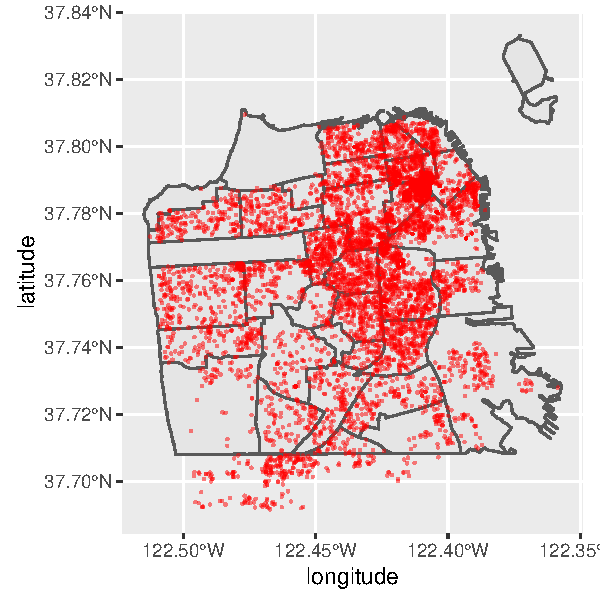
\includegraphics[width=\maxwidth]{figure/chunk-plotPlace-1} \end{marginfigure}

\end{knitrout}
Inesperadamente, o mapa mostra alguns pontos de alojamento fora da cidade, mas julgamos que não vá interferir com as nossas análises, devido ao correto agrupamento\sidenote{Demonstrado mais à frente.} e à proximidade da cidade. Embora a razão nos seja desconhecida, acreditamos que o próprio Airbnb agrupa desta forma esses locais devido à sua proximidade com a cidade. \\
A concentração torna-se mais óbvia quando visualizamos o mapa de calor.
\begin{knitrout}
\definecolor{shadecolor}{rgb}{0.969, 0.969, 0.969}\color{fgcolor}\begin{kframe}
\begin{alltt}
\hlstd{rast} \hlkwb{<-} \hlstd{(shape_plot} \hlopt{+} \hlkwd{stat_bin2d}\hlstd{(}\hlkwc{data} \hlstd{= df,}
    \hlkwd{aes}\hlstd{(}\hlkwc{x} \hlstd{= longitude,} \hlkwc{y} \hlstd{= latitude),}
    \hlkwc{alpha} \hlstd{=} \hlnum{0.7}\hlstd{,} \hlkwc{bins} \hlstd{=} \hlnum{30}\hlstd{,}
    \hlkwc{linejoin} \hlstd{=} \hlstr{"round"}\hlstd{)} \hlopt{+}
    \hlkwd{scale_fill_viridis_c}\hlstd{(}\hlkwc{option} \hlstd{=} \hlstr{"C"}\hlstd{))}
\hlstd{rast}
\end{alltt}
\end{kframe}\begin{marginfigure}
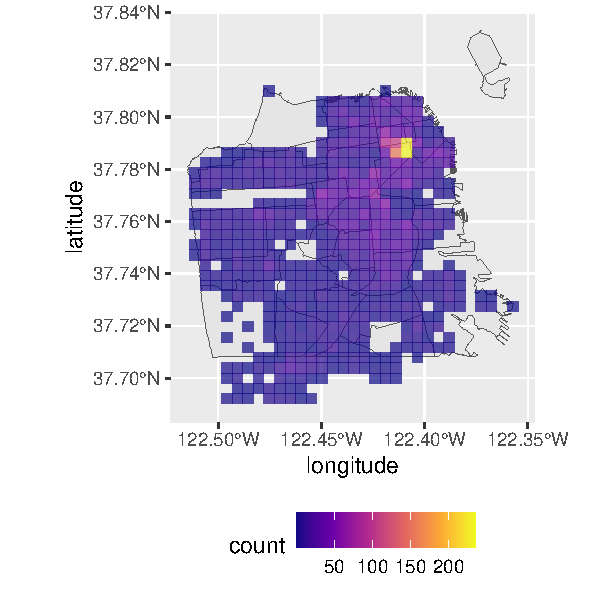
\includegraphics[width=\maxwidth]{figure/chunk-rasterPlaces-1} \end{marginfigure}

\end{knitrout}
\begin{knitrout}
\definecolor{shadecolor}{rgb}{0.969, 0.969, 0.969}\color{fgcolor}\begin{kframe}
\begin{alltt}
\hlcom{# rast %>% extractLegend}
\end{alltt}
\end{kframe}
\end{knitrout}
O mapa claramente demonstra a concentração de alojamentos na zona clara, mas também consegue-se observar uma grande quantidade, embora mais dispersos, na zona central.
\begin{knitrout}
\definecolor{shadecolor}{rgb}{0.969, 0.969, 0.969}\color{fgcolor}\begin{kframe}
\begin{alltt}
\hlstd{df} \hlopt
    \hlkwd{group_by}\hlstd{(neighbourhood)} \hlopt
    \hlkwd{summarise}\hlstd{(}\hlkwc{n} \hlstd{=} \hlkwd{n}\hlstd{(),} \hlkwc{freq} \hlstd{= n}\hlopt{/}\hlkwd{nrow}\hlstd{(df))} \hlopt
    \hlkwd{arrange}\hlstd{(}\hlopt{-}\hlstd{n)} \hlopt
    \hlkwd{head}\hlstd{(}\hlnum{8}\hlstd{)} \hlopt
    \hlkwd{showT}\hlstd{()}
\end{alltt}
\end{kframe}\begingroup\fontsize{10}{12}\selectfont

\begin{RTable}{r|r|r}
\hline
neighbourhood & n & freq\\
\hline
\cellcolor{gray!6}{Downtown/Civic Center} & \cellcolor{gray!6}{745} & \cellcolor{gray!6}{0.1123850}\\
\hline
Mission & 558 & 0.0841756\\
\hline
\cellcolor{gray!6}{South of Market} & \cellcolor{gray!6}{450} & \cellcolor{gray!6}{0.0678835}\\
\hline
Western Addition & 418 & 0.0630563\\
\hline
\cellcolor{gray!6}{Nob Hill} & \cellcolor{gray!6}{328} & \cellcolor{gray!6}{0.0494796}\\
\hline
Outer Sunset & 281 & 0.0423895\\
\hline
\cellcolor{gray!6}{Bernal Heights} & \cellcolor{gray!6}{280} & \cellcolor{gray!6}{0.0422386}\\
\hline
Haight Ashbury & 276 & 0.0416352\\
\hline
\end{RTable}
\endgroup{}

\end{knitrout}
A tabela mostra que a maioria dos alojamentos listados estão localizados no distrito de \textit{Downtown/Civic Center} e \textit{Mission}.

\begin{knitrout}
\definecolor{shadecolor}{rgb}{0.969, 0.969, 0.969}\color{fgcolor}\begin{kframe}
\begin{alltt}
\hlstd{shape_plot} \hlopt{+} \hlkwd{geom_point}\hlstd{(}\hlkwc{data} \hlstd{= df,}
    \hlkwd{aes}\hlstd{(}\hlkwc{y} \hlstd{= latitude,} \hlkwc{x} \hlstd{= longitude,}
        \hlkwc{color} \hlstd{= neighbourhood),}
    \hlkwc{alpha} \hlstd{=} \hlnum{0.5}\hlstd{,} \hlkwc{size} \hlstd{=} \hlnum{0.1}\hlstd{)} \hlopt{+}
    \hlkwd{geom_point}\hlstd{(}\hlkwc{data} \hlstd{= (df} \hlopt
        \hlkwd{filter}\hlstd{(neighbourhood} \hlopt{==}
            \hlstr{"Downtown/Civic Center"}\hlstd{)),}
        \hlkwd{aes}\hlstd{(}\hlkwc{y} \hlstd{= latitude,}
            \hlkwc{x} \hlstd{= longitude),}
        \hlkwc{color} \hlstd{=} \hlstr{"red"}\hlstd{,} \hlkwc{alpha} \hlstd{=} \hlnum{1}\hlstd{,}
        \hlkwc{size} \hlstd{=} \hlnum{0.1}\hlstd{)} \hlopt{+} \hlkwd{theme}\hlstd{(}\hlkwc{legend.position} \hlstd{=} \hlstr{"none"}\hlstd{)}
\end{alltt}
\end{kframe}\begin{marginfigure}
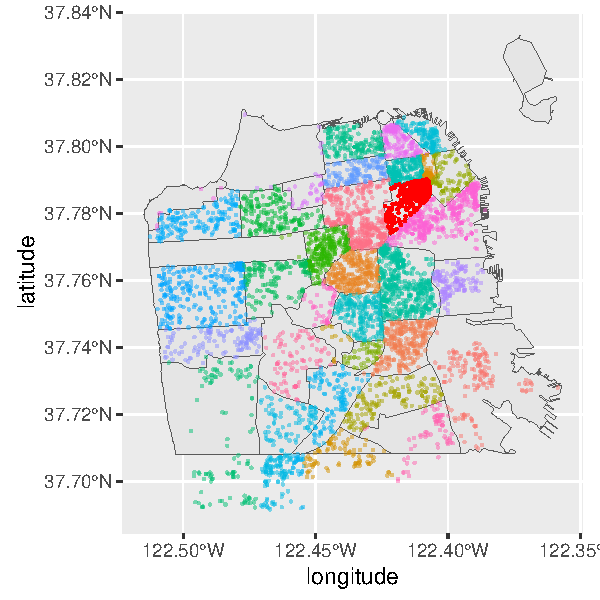
\includegraphics[width=\maxwidth]{figure/chunk-plotNeighbs-1} \end{marginfigure}

\end{knitrout}
Este gráfico demonstra que os bairros conformem com a definição do Departamento de Planejamento da cidade. Demonstra também a posição do distrito \textit{Downtown/Civic Center} a vermelho, conforme o mapa de calor. \pagebreak

\begin{knitrout}
\definecolor{shadecolor}{rgb}{0.969, 0.969, 0.969}\color{fgcolor}\begin{kframe}
\begin{alltt}
\hlstd{pricePlot} \hlkwb{<-} \hlkwd{ggplot}\hlstd{(}\hlkwc{data} \hlstd{= df,}
    \hlkwd{aes}\hlstd{(price))}
\hlstd{pricebox} \hlkwb{<-} \hlstd{pricePlot} \hlopt{+} \hlkwd{geom_boxplot}\hlstd{()} \hlopt{+}
    \hlkwd{coord_flip}\hlstd{()}
\hlstd{pricebox}
\end{alltt}
\end{kframe}\begin{marginfigure}
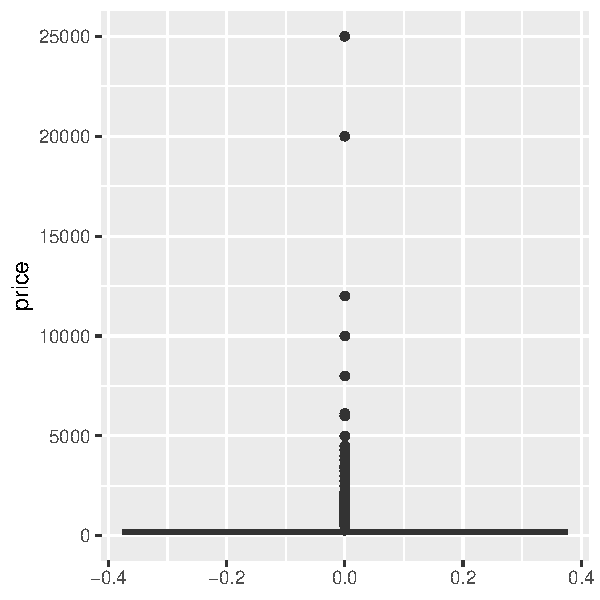
\includegraphics[width=\maxwidth]{figure/chunk-priceBoxPlot-1} \end{marginfigure}

\end{knitrout}
Este \textit{boxplot} do preço consegue notar imediatamente a existem de muitos valores atípicos, o que equivalem a preços muito altos, comparado com a média de preços dos registos, 303.465 USD. Estes preços vão sem dúvida interferir com as nossas análises. \\
Estes preços conseguem ser justificados quando analisamos a fonte destes preços altos.
\begin{knitrout}
\definecolor{shadecolor}{rgb}{0.969, 0.969, 0.969}\color{fgcolor}\begin{kframe}
\begin{alltt}
\hlstd{df} \hlopt
    \hlkwd{select}\hlstd{(name, price)} \hlopt
    \hlkwd{arrange}\hlstd{(}\hlopt{-}\hlstd{price)} \hlopt
    \hlkwd{head}\hlstd{(}\hlnum{7}\hlstd{)} \hlopt
    \hlkwd{showT}\hlstd{(T)}
\end{alltt}
\end{kframe}\begingroup\fontsize{10}{12}\selectfont

\begin{RTable*}{r|r}
\hline
name & price\\
\hline
\cellcolor{gray!6}{Harbor Court Hotel, Bay View King Room} & \cellcolor{gray!6}{25000}\\
\hline
Harbor Court Hotel, Bay View Queen Room & 25000\\
\hline
\cellcolor{gray!6}{Hotel Griffon by the Bay, queen bedded room} & \cellcolor{gray!6}{25000}\\
\hline
1-Bedroom Suite with One Bed and One Sofabed at Fairmont San Francisco by Suiteness & 20000\\
\hline
\cellcolor{gray!6}{Suite plus Connecting Room with Three Beds and One Sofabed at Fairmont San Francisco by Suiteness} & \cellcolor{gray!6}{20000}\\
\hline
Suite plus Connecting Room with Two Beds and One Sofabed at Fairmont San Francisco by Suiteness & 20000\\
\hline
\cellcolor{gray!6}{1-Bedroom Suite with One Bed at Fairmont San Francisco by Suiteness} & \cellcolor{gray!6}{20000}\\
\hline
\end{RTable*}
\endgroup{}

\end{knitrout}

Estes preços equivalem a alojamentos de luxo. Estes alojamentos vão ter que ser tratadas de forma diferente quando a for feita a modelação, pois não são comparáveis com o resto dos alojamentos. Por agora, de forma a poder analisar a maioria dos alojamentos, vamos apenas ver a preços abaixo de 895 USD. \\

\begin{knitrout}
\definecolor{shadecolor}{rgb}{0.969, 0.969, 0.969}\color{fgcolor}\begin{kframe}
\begin{alltt}
\hlstd{upper_limit} \hlkwb{<-} \hlkwd{quantile}\hlstd{(df}\hlopt{$}\hlstd{price,}
    \hlnum{0.975}\hlstd{)} \hlopt{+} \hlnum{20}
\hlstd{pricebox} \hlopt{+} \hlkwd{xlim}\hlstd{(}\hlnum{0}\hlstd{, upper_limit)}
\end{alltt}
\end{kframe}\begin{marginfigure}
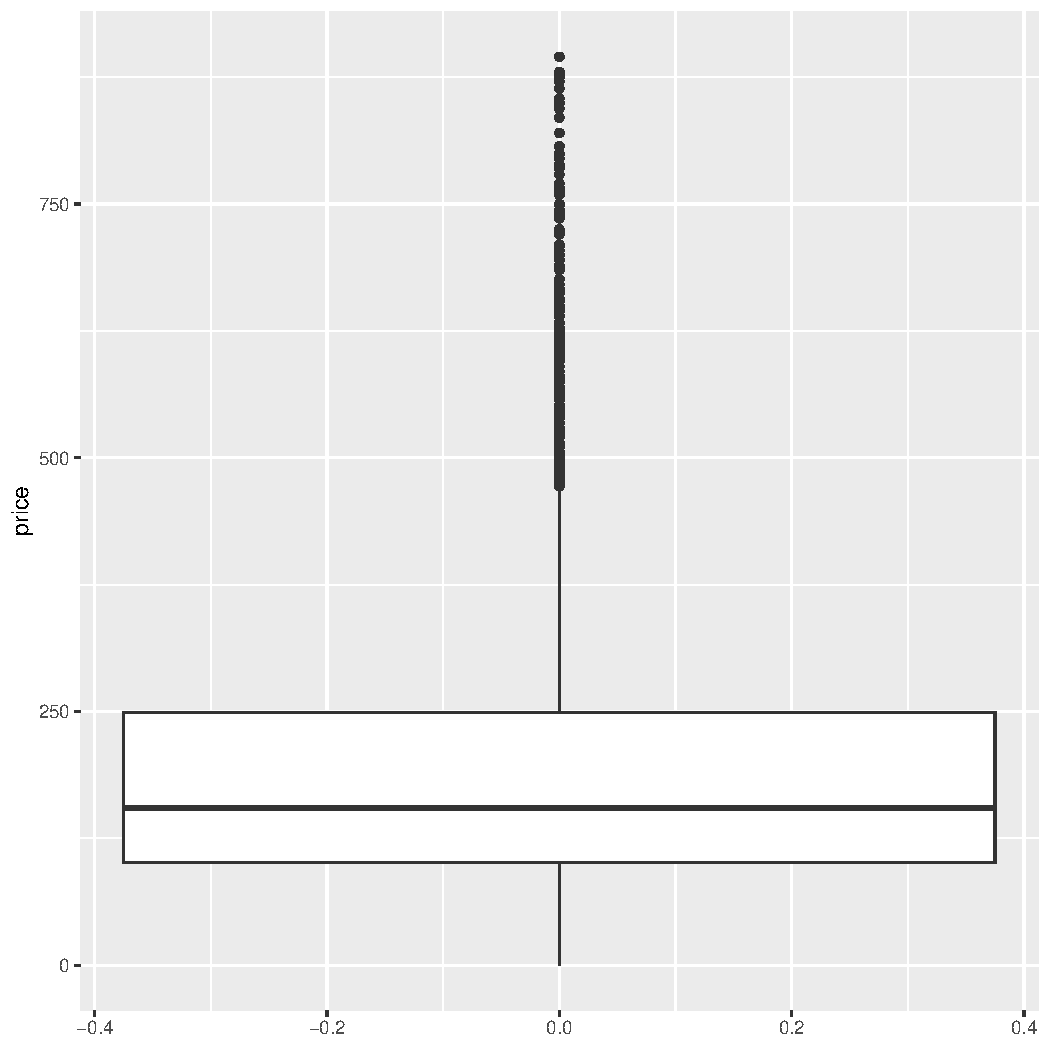
\includegraphics[width=\maxwidth]{figure/chunk-priceBoxPlotLim-1} \end{marginfigure}

\end{knitrout}
Este \textit{boxplot} mostra que a maioria dos alojamentos tem preços entre 103 e 254 USD. Este facto torna-se ainda mais evidente quando analisamos a distribuição dos preços. \\
O gráfico mostra também que há muitos alojamentos fora destes limites, podendo ser valores atípicos também, embora não tão extremos como aqueles vistos anteriormente. No entanto, à primeira vista estes não devem ser valores atípicos, devido à sua quantidade, mesmo quando comparado com o número de registos.\\

\begin{knitrout}
\definecolor{shadecolor}{rgb}{0.969, 0.969, 0.969}\color{fgcolor}\begin{kframe}
\begin{alltt}
\hlstd{pricePlot} \hlopt{+} \hlkwd{geom_histogram}\hlstd{(}\hlkwc{binwidth} \hlstd{=} \hlnum{25}\hlstd{,}
    \hlkwd{aes}\hlstd{(}\hlkwc{y} \hlstd{= ..density..))} \hlopt{+}
    \hlkwd{geom_density}\hlstd{(}\hlkwc{color} \hlstd{=} \hlstr{"red"}\hlstd{)} \hlopt{+}
    \hlkwd{xlim}\hlstd{(}\hlnum{0}\hlstd{, upper_limit)}
\end{alltt}
\end{kframe}\begin{marginfigure}
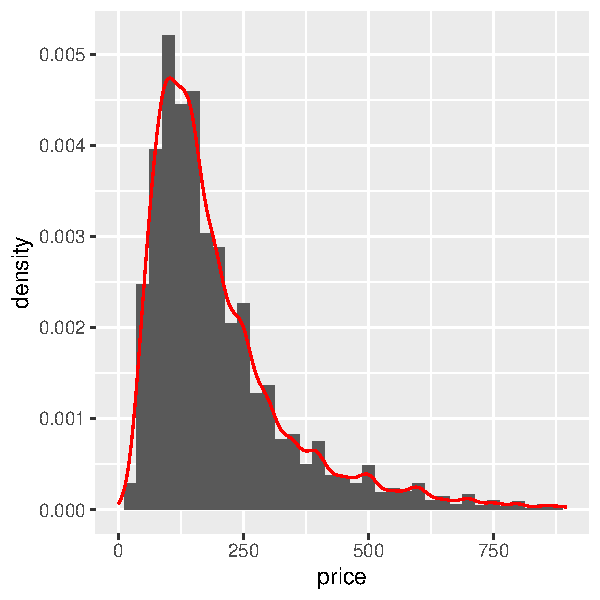
\includegraphics[width=\maxwidth]{figure/chunk-priceHist-1} \end{marginfigure}

\end{knitrout}
A distribuição de preços apresentada demonstra que a maioria dos alojamentos se encontram no limite mostrado anteriormente, e a distribuição parece aproximar-se de uma distribuição $\chi_{k}^{2}$, com um pequeno grau de liberdade. Curiosamente, o gráfico mostra que os preços parecem aumentar algumas vezes cada 50 USD, o que pode ser devido ao facto de que os hospedeiros escolhem preços redondos, como 50, 100, 175, etc. Este fenómeno parece ser mais visível nos 250 e nos 500.\\

\begin{knitrout}
\definecolor{shadecolor}{rgb}{0.969, 0.969, 0.969}\color{fgcolor}\begin{kframe}
\begin{alltt}
\hlstd{df} \hlopt
    \hlkwd{ggplot}\hlstd{(}\hlkwd{aes}\hlstd{(}\hlkwc{x} \hlstd{= price,}
        \hlkwc{y} \hlstd{=} \hlkwd{fct_reorder}\hlstd{(neighbourhood,}
            \hlopt{-}\hlstd{price,} \hlkwc{.fun} \hlstd{= median)))} \hlopt{+}
    \hlkwd{geom_boxplot}\hlstd{()} \hlopt{+} \hlkwd{xlim}\hlstd{(}\hlnum{0}\hlstd{,}
    \hlstd{upper_limit)} \hlopt{+} \hlkwd{labs}\hlstd{(}\hlkwc{y} \hlstd{=} \hlstr{""}\hlstd{)}
\end{alltt}
\end{kframe}\begin{figure*}
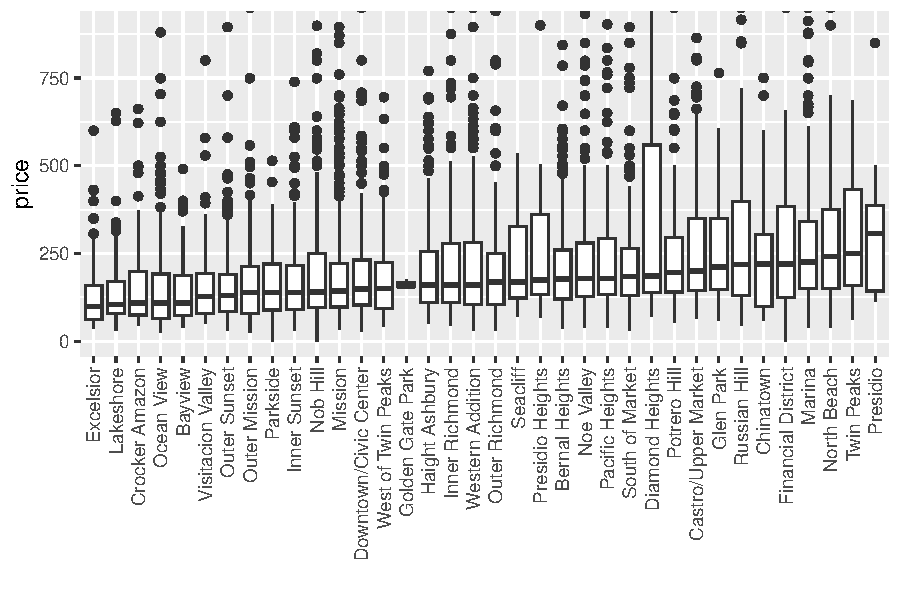
\includegraphics[width=\maxwidth]{figure/chunk-boxPriceNeighs-1} \end{figure*}

\end{knitrout}
Os \textit{boxplots} mostram que os preços dos alojamentos não variam bastante de acordo com o bairro sendo que o ponto médio não varia bastante entre bairros, excepto os bairros \textit{Twin Peaks}, e \textit{Presidio}. No entanto, o gráfico mostra uma grande variância dos preços em todos os bairros.\\

\begin{knitrout}
\definecolor{shadecolor}{rgb}{0.969, 0.969, 0.969}\color{fgcolor}\begin{kframe}
\begin{alltt}
\hlstd{df} \hlopt
    \hlkwd{group_by}\hlstd{(room_type)} \hlopt
    \hlkwd{summarise}\hlstd{(}\hlkwc{n} \hlstd{=} \hlkwd{n}\hlstd{(),} \hlkwc{freq} \hlstd{=} \hlkwd{n}\hlstd{()}\hlopt{/}\hlkwd{nrow}\hlstd{(.),}
        \hlkwc{averagePrice} \hlstd{=} \hlkwd{mean}\hlstd{(price))} \hlopt
    \hlkwd{showT}\hlstd{()}
\end{alltt}
\end{kframe}\begingroup\fontsize{10}{12}\selectfont

\begin{RTable}{r|r|r|r}
\hline
room\_type & n & freq & averagePrice\\
\hline
\cellcolor{gray!6}{Entire home/apt} & \cellcolor{gray!6}{4243} & \cellcolor{gray!6}{0.6400664} & \cellcolor{gray!6}{275.8965}\\
\hline
Hotel room & 65 & 0.0098054 & 266.2154\\
\hline
\cellcolor{gray!6}{Private room} & \cellcolor{gray!6}{2239} & \cellcolor{gray!6}{0.3377583} & \cellcolor{gray!6}{360.1474}\\
\hline
Shared room & 82 & 0.0123699 & 211.7683\\
\hline
\end{RTable}
\endgroup{}

\end{knitrout}
A tabela mostra que a maioria dos alojamentos são apartamentos ou casas inteiras, enquanto que os quartos privados são menos frequents. Mostra também a pequena quantidade de quartos de hoteis e de alojamentos partilhados, sendo estes apenas $2\%$ dos registos. A tablea também expoem que os quartos privados são os mais caros em média, enquanto que os alojamentos partilhados são os mais baratos. Enquanto que o preço médio das salas partilhadas é esperado, é supreendente que os quartos privados sejam mais caros em média que as casas inteiras e os quartos de hotel. Isto pode ser porque a diferença entre "quarto privado" e "quarto de hotel" pode ser confusa, tanto que os hoteis de alto preço notados em cima estão caracterizados como "quartos privados".\\
\begin{knitrout}
\definecolor{shadecolor}{rgb}{0.969, 0.969, 0.969}\color{fgcolor}\begin{kframe}
\begin{alltt}
\hlstd{df} \hlopt
    \hlkwd{group_by}\hlstd{(room_type)} \hlopt
    \hlkwd{filter}\hlstd{(price} \hlopt{<} \hlstd{upper_limit)} \hlopt
    \hlkwd{summarise}\hlstd{(}\hlkwc{n} \hlstd{=} \hlkwd{n}\hlstd{(),} \hlkwc{freq} \hlstd{=} \hlkwd{n}\hlstd{()}\hlopt{/}\hlkwd{nrow}\hlstd{(.),}
        \hlkwc{averagePrice} \hlstd{=} \hlkwd{mean}\hlstd{(price))} \hlopt
    \hlkwd{showT}\hlstd{()}
\end{alltt}
\end{kframe}\begingroup\fontsize{10}{12}\selectfont

\begin{RTable}{r|r|r|r}
\hline
room\_type & n & freq & averagePrice\\
\hline
\cellcolor{gray!6}{Entire home/apt} & \cellcolor{gray!6}{4131} & \cellcolor{gray!6}{0.6388803} & \cellcolor{gray!6}{233.9990}\\
\hline
Hotel room & 63 & 0.0097433 & 241.0159\\
\hline
\cellcolor{gray!6}{Private room} & \cellcolor{gray!6}{2192} & \cellcolor{gray!6}{0.3390040} & \cellcolor{gray!6}{135.2176}\\
\hline
Shared room & 80 & 0.0123724 & 78.3125\\
\hline
\end{RTable}
\endgroup{}

\end{knitrout}

Se excluirmos os apartamentos de luxo, conseguimos observar valores mais esperados; quartos de hoteis serem os mais caros com preços aproximados aos das casas inteiras, e os alojamentos partilhados serem os mais baratos. Os preços médios dos quartos privados desceram significativamente, e isto pode ser explicado pela classificação de alojamentos de luxo como "quartos privados". Nós suspeitamos que, sem os quartos de luxo, esta nova categoria identifica-se mais com albergues.\\

\begin{knitrout}
\definecolor{shadecolor}{rgb}{0.969, 0.969, 0.969}\color{fgcolor}\begin{kframe}
\begin{alltt}
\hlkwd{ggplot}\hlstd{(df,} \hlkwd{aes}\hlstd{(}\hlkwc{x} \hlstd{= price,}
    \hlkwc{y} \hlstd{= room_type,} \hlkwc{fill} \hlstd{= room_type))} \hlopt{+}
    \hlkwd{geom_density_ridges}\hlstd{()} \hlopt{+}
    \hlkwd{xlim}\hlstd{(}\hlnum{0}\hlstd{, upper_limit)} \hlopt{+}
    \hlkwd{theme_ridges}\hlstd{()} \hlopt{+} \hlkwd{theme}\hlstd{(}\hlkwc{legend.position} \hlstd{=} \hlstr{"none"}\hlstd{)}
\end{alltt}
\end{kframe}\begin{marginfigure}
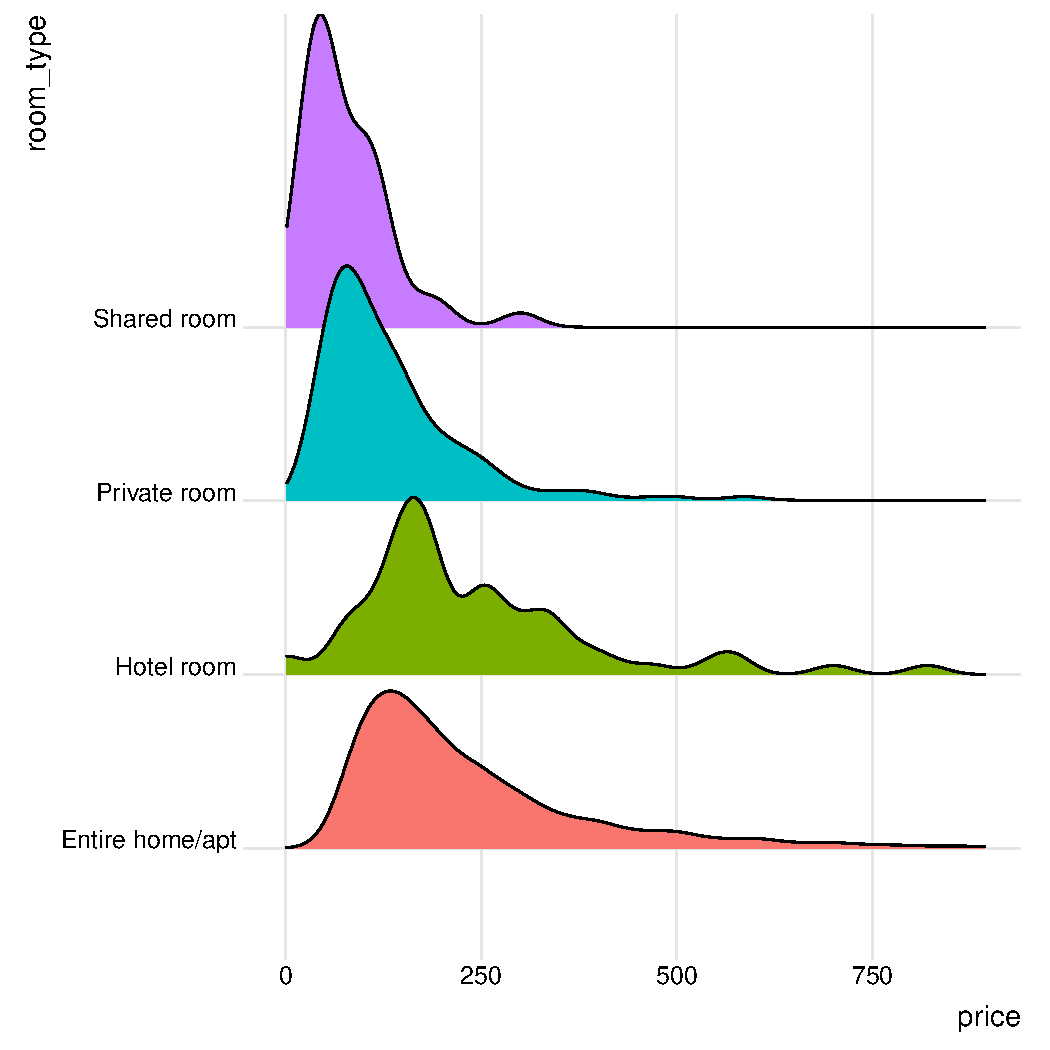
\includegraphics[width=\maxwidth]{figure/chunk-RoomTypesPrice-1} \end{marginfigure}

\end{knitrout}

O diagrama apresentado demonstra as distribuições dos preços por tipo de alojamento. Ele corrobora que os quartos de hóteis sejam os mais caros, mas parece demonstrar que a maioria dos outros grupos se encontram com preços semelhantes, com uma diferença na densidade na cauda do gráfico, explicando assim a alta média de apartamentos inteiros; ou seja, a maioria dos alojamentos inteiros estão de acordo com quartos privados, mas existem mais alojamentos inteiros mais caros.

\begin{knitrout}
\definecolor{shadecolor}{rgb}{0.969, 0.969, 0.969}\color{fgcolor}\begin{kframe}
\begin{alltt}
\hlkwd{ggcorrplot}\hlstd{(}\hlkwd{cor}\hlstd{(df} \hlopt
    \hlkwd{select}\hlstd{(latitude, longitude,}
        \hlstd{price, reviews_per_month,}
        \hlstd{availability_365,}
        \hlstd{number_of_reviews_ltm),}
    \hlkwc{use} \hlstd{=} \hlstr{"complete.obs"}\hlstd{),}
    \hlkwc{lab} \hlstd{=} \hlnum{TRUE}\hlstd{)}
\end{alltt}
\end{kframe}\begin{figure*}
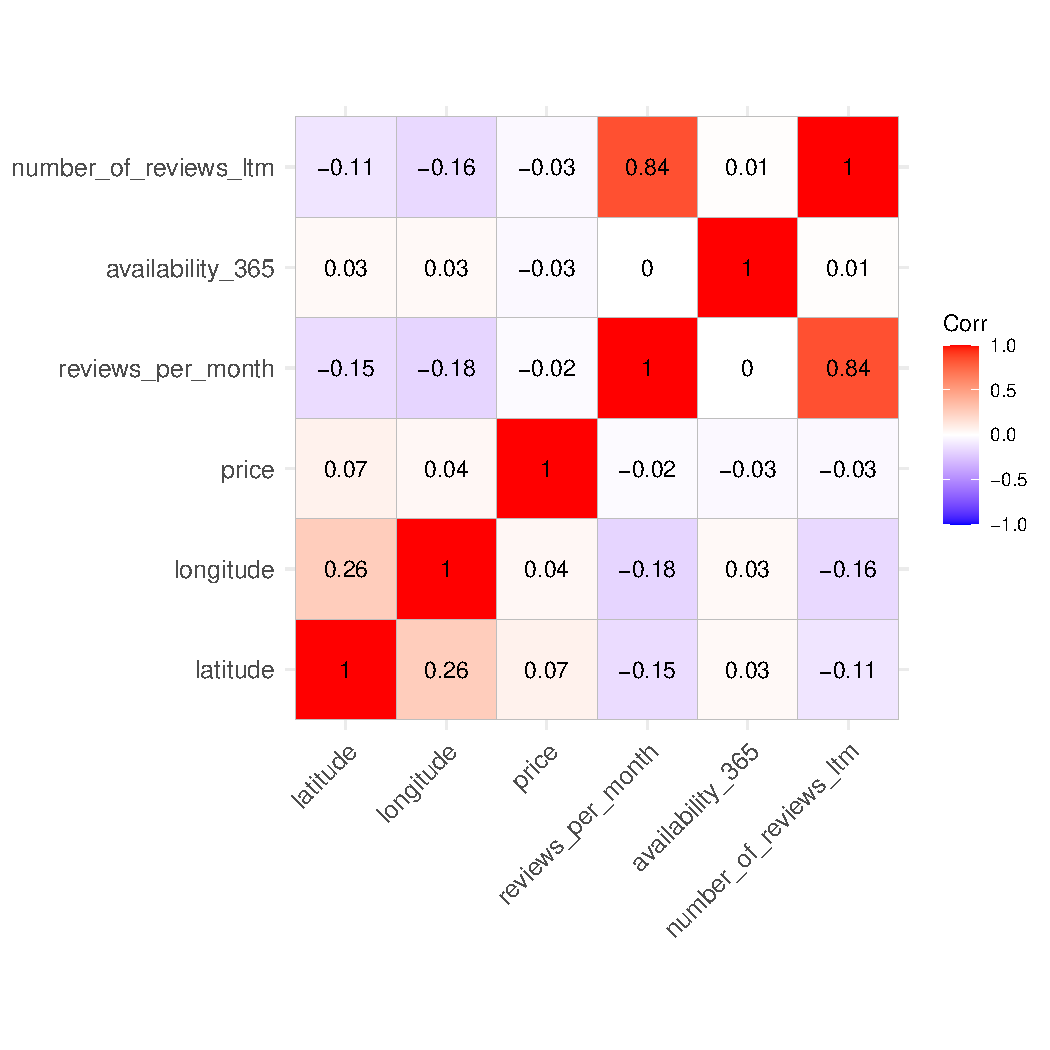
\includegraphics[width=\maxwidth]{figure/chunk-CorrPlot-1} \end{figure*}

\end{knitrout}

\nobibliography{references.bib}
\bibliographystyle{plainnat}
\end{document}
